\section{Structure of a Colony}\label{sec:colony-structure}
Colonies exist to enable collaboration between their members, and direct collective efforts towards common goals. Facilitating effective division of labour, management of incentives, and allocation of resources are therefore some of the most important functions of the Colony protocol.

\subsection{Domains and permissions}\label{sec:domains}\label{sec:permissions}

The essential structure of the colony revolves around domains and the permissions that accounts may have in them. These two concepts jointly define the structure and security of a colony and provide a flexible framework for creating colonies of many kinds.

\subsubsection{Domains}

Like any organization, without structure, a large colony would quickly become difficult to navigate due to the sheer number of participants and interactions taking place --- domains solve this problem. A domain is like a folder in a shared filesystem, except instead of containing files and folders, it can contain subdomains, funding, and expenditures. This simple modularity enables great flexibility as to how an organisation may be structured. Domains could be used to represent teams, departments, projects, tribes, circles, and so forth. A toy example is shown in in Figure \ref{fig:domainhierarchysample}.

\begin{figure}[h]
    \centering
 \begin{tikzpicture}
   \node[shape=ellipse, draw] at (0,0) (tld) {Root};

   \node[shape=ellipse, draw] at (-3,-2) (design) {Design}
    (tld) edge[-] (design);

   \node[shape=ellipse, draw] at (0,-2) (development) {Development}
    (tld) edge[-] (development);

   \node[shape=ellipse, draw] at (3,-2) (product) {Product}
    (tld) edge[-] (product);

   \node[shape=ellipse, draw] at (-1.5,-4) (frontend) {Frontend}
    (development) edge[-] (frontend);

   \node[shape=ellipse, draw] at (1.5,-4) (backend) {Backend}
    (development)  edge[-] (backend);
 \end{tikzpicture}
 \caption{Parts of a domain hierarchy for a colony developing a web service.}
 \label{fig:domainhierarchysample}
\end{figure}

It is ultimately up to individual colonies to decide how they wish to use domains—some might only use them for coarse categorisations, whereas others may use them to precisely group only the most similar expenditures together, or even multiple expenditures that other colonies would consider a single expenditure. Some might use domains to represent long-lived organizational departments, while others might use them more ephemerally, to represent projects with start and end dates. We aim to provide a general framework that colonies may use however they see fit, and to be prescriptive only where necessary.

Among other things, this compartmentalisation of activity provides an essential benefit to the colony as a whole by making reputation \textit{contextual}. When arbitration occurs, it occurs at a specific level in the colony's domain hierarchy. This means that people with relevant contextual knowledge can be included for their opinion, and that when arbitration occurs, the whole colony is not required to participate in the process.

\subsubsection{Permissions}

Access control in a colony is organized around the concepts of \textbf{permissions}. There are six different permissions (roughly in order of influence): recovery, root, arbitration, architecture, funding, and arbitration, each unlocking a bundle of semantically-related functionality.

With the exception of the recovery and root permissions, all permissions are domain-specific (much like permissions in a Unix file system are directory-specific), with the rule that permissions held in a parent domain are inherited in all child domains. Put another way, have a permission in a domain gives you that permission in the entire \textit{subtree} rooted in that domain. To implement this inheritance, permissioned functions require a \textit{domain proof} of the following arguments:

\begin{itemize}
\item \texttt{permissionDomainId} - The (parent) domain in which the account holds the permission.
\item \texttt{childSkillIndex} - The index of \texttt{domainId} in \texttt{permissionDomainId}'s \texttt{children} array.
\item \texttt{domainId} - The (child) domain in which the action is being taken.
\end{itemize}

These arguments can be evaluated on-chain in constant time to determine whether the account is authorized to call the privileged function.

Permissions are held by Ethereum accounts. This means that permissions may be given to human administrators, or assigned to contracts which implement more complex behavior (such as voting mechanisms). These types of contracts are known as \textbf{extensions} and are discussed in-depth in Section \ref{sec:extensions}. The use of extensions to flexibly `plug-in' various decision-making mechanisms is a key concept in the Colony protocol.

It is worth noting that the list of accounts that have the permission in question have the full permission; no additional restrictions exist at the protocol level. In some cases, these are extremely powerful capabilities (such as emitting arbitrary reputation penalties) and require absolute confidence in whomever or whatever controls it. We anticipate therefore that in many cases, extension contracts will be used to offer varying degree of moderation to the underlying permissions.

\subsubsection*{Recovery}

The recovery permission gives accounts access to the colony's emergency `recovery' functionality, which allows for arbitrary state-changes to the colony's data. Recovery mode is described in more detail in Section \ref{sec:escape-hatches}.

\subsubsection*{Root}

The root permission gives accounts access to high-level administrative functions in the colony, such as setting colony-wide parameters, upgrading the colony, and minting new internal tokens. This permission also gives accounts the ability to assign permissions throughout the colony (including in the root domain).

\subsubsection*{Arbitration}

The arbitration permission gives accounts the ability to make domain-specific state changes, meant as a means of resolving motions. This permission also enables accounts to emit reputation penalties (but not reputation increases).

\subsubsection*{Architecture}

The architecture permission gives accounts the ability to create new domains in a colony, as well as assign permissions in those new domains. Unlike root, accounts with this permission cannot edit permissions in the domain in which they hold the permission, only in subdomains.

\subsubsection*{Funding}

The funding permission gives accounts the ability to move tokens between funding pots. In practice, this means that this permission is responsible for allocating money amongst domains and for funding expenditures. Financial management in a colony is described in more detail in Section \ref{sec:finance}.

\subsubsection*{Administration}

The administration permission gives accounts the ability to create and manage (but not fund) expenditures, the basic incentive unit in a colony, described in Section \ref{sec:expenditures}. \\

Broadly, permissions are designed as a `separation of powers': different permissions must work in concert to carry out the functioning of a colony. For example, administration can create an expenditure, but only funding can actually provide the resources, while arbitration resolves motions as they arise. Complex extensions may require multiple permissions in order to function properly (such as `tasks', which requires both arbitration and administration).

The intention is that, since permissions are grouped into semantic bundles of functionality, it will be possible to develop \textit{specialized} mechanisms for mediating access to the underlying functionality (i.e. specialized funding mechanisms and specialized dispute-resolution mechanisms, as opposed to a general-purpose `voting' mechanism meant to handle all possible decisions).

Colony's long-term vision is of \textit{trustless organizations}; organizations in which members can safely collaborate and manage shared resources, without needing to know or trust each other. Early colonies may find that a larger emphasis on human moderators to be useful, while more mature colonies may find reasons to devolve increasingly more decision-making to extensions implementing trustless functionality. We will refer to colonies which make substantial use of these extensions as \textit{trustless colonies}.

\subsection{Funding and expenditures}\label{sec:expenditures}\label{sec:finance}

All tokens and currencies are administered by the colony contract; it is responsible for all the bookkeeping and allocations. The former are managed via funding pots, the latter via expenditures.

\subsubsection{Funding pots}

Each domain and each expenditure in a colony has an associated \emph{funding pot}. A funding pot can be thought of as a wallet specific to a particular domain or expenditure, and are used to move funds around \textit{within} a colony. To each funding pot, the colony contract may associate any number of Ether or ERC20-compatible tokens it holds. Depending on context, the funds in a funding pot may be referred to as the payout, bounty, budget, salary or working capital. In addition to the funding pots, there is a special \emph{rewards pot} which accumulates tokens to be distributed to members as \textit{rewards} (see Section \ref{sec:revenue}).

Only accounts holding the \textbf{funding} permission may move tokens; the rule is that they may move tokens between any two pots in the subtree rooted in the domain in which they hold the permission. It is the expectation that this permission will in many cases be given to an \textit{extension contract} implementing a specialized decision-making mechanism, such as the \textit{funding queue} described in Section \ref{sec:funding-queues}.

\subsubsection{Expenditures}

The basic payment primitive of a colony is the `expenditure'. Expenditures are used to transfer funds out of a colony to any Ethereum account. An expenditure has several properties:

\begin{itemize}
\item An \texttt{owner} (the account address which created the expenditure).
\item A \texttt{status} (active, cancelled, or finalized).
\item One or more \texttt{recipient}s.
\item \texttt{payouts} for each recipient, denominated in one or more tokens.
\item Optionally, a per-recipient \texttt{skill}.
\item Optionally, a per-recipient \texttt{payoutModifier}.
\item Optionally, a per-recipient \texttt{claimDelay}.
\end{itemize}

The owner is responsible for setting the properties of the expenditure. The recipients are simply Ethereum accounts. While it is anticipated that recipients will be individuals, there is nothing to prevent these accounts being contracts under the control of multiple people.\footnote{With the protocol as described in this document, any reputation earned would be assigned to the contract in question and not able to be moved to the appropriate users. In these cases, it might be better to develop an extension contract which would determine the per-user allocation in advance and configure the expenditure accordingly.}

Once the expenditure is finalized, all properties become locked (but subject to arbitration) and payouts can be claimed (and reputation awarded). Prior to finalization, the owner has the ability to cancel the expenditure entirely. Any funds that have already been assigned to the expenditure can be reassigned to the domain that the expenditure was created in.

Defining the payouts for each recipient, of course, does not provide the funds --- this must be done through the funding mechanisms in Colony. Payouts do not have to all be in the same token, and an expenditure's payouts can be made up of an arbitrary number of tokens.

The expenditure is meant to be an abstract primitive which can support many types of workflows, and so contains optional attributes to support more complex behavior (see Section \ref{sec:extensions}). For instance, the \texttt{payoutModifier} and \texttt{claimDelay} can be used to implement a rating and review system, where good or bad reviews lead to an across-the-board reputation increase (or payout decrease) for a recipient, while the \texttt{claimDelay} is set to allow for any relevant motions to be decided before funds can exit the colony. \\

Once the tokens have been received by an account, they are under the control of the recipient --- there is no way to reclaim the funds. The funds have to cross the `Cryptographic Rubicon' somewhere in the system (by the nature of the blockchain), and it makes sense to do so here.\footnote{Currently, the only way this rule can be broken is by the Colony conspiring to abuse the `arbitrary transaction' feature described in Section \ref{sec:arbitrary-transaction}.}

\subsection{Internal tokens}\label{sec:colony-tokens}

Every colony has its own ERC20-compatible `internal token'. These are the tokens that, when earned as an expenditure payout, also generate reputation for the receiver (and thus distribute control within the colony). What these tokens represent apart from this is up to the colony to decide. For example, they may have financial value, or they may be purely symbolic; some possible scenarios are outlined in this section.

In addition, colonies may `bring their own token' and designate an existing ERC20-compatible token as reputation-bearing. While this may be advantageous in some contexts, it’s worth noting that this weakens the incentive alignment underpinning the game theoretic security of trustless colonies, in that the value of the token is divorced from the performance of the colony. Note that the internal token cannot be changed once a colony has been created, so \textit{choose wisely}.

In cases where a colony creates a new token, that colony is in control of the supply of the token. Specifically, \textbf{root} permission holders can mint tokens at-will. In some cases, this may look like a founder managing the token supply unilaterally, while in other cases colonies may manage the minting process via an extension contract (see Section \ref{sec:colony-token-management} for an example).

A common question is why only internal tokens (as opposed to all tokens) are reputation-bearing. The reason for having a single token be reputation-bearing is that it avoids tricky exchange-rate problems, such as incentives to receive more of a less valuable token to earn more reputation.

\subsubsection{Token use-cases}

Ultimately, internal tokens are used to distribute reputation, and thus both ownership and decision-making power. Since users with more reputation can both exercise more influence over the activity of the colony, as well as claim a greater share of the rewards, reputation functions to align incentives among the members of colony. Here we give a few examples of different use-cases for internal tokens, demonstrating the variety of schemes colonies may adopt for distributing ownership and influence alongside cash compensation.

\subsubsection*{Tokens as early rewards}

One of the chief benefits of a colony having its own token is that it can offer rewards for work before it has any revenue or external funding to draw on. A new colony may offer token payouts for expenditures with the hope that the reputation earned by these token payments (and the future revenue earned by the colony) will eventually lead to financial rewards. By allowing `spending' before fund-raising, the financial burden during the start-up phase of a new colony is eased. Once a colony is profitable, payment in tokens may be the exception rather than the norm.

\subsubsection*{Tokens representing hours worked}

We could imagine a colony in which all expenditures are paid in Ether, but include a number of the colony's own tokens as well, equal to the expected number of hours worked. The members of the colony would be responsible for assigning `correct' token and Ether payouts to expenditures. This extra responsibility would also ensure users doing the same amount of work received the same reputation gain, rather than the reputation gain being dependent on the rates they charged.

\subsubsection*{Tokens as performance-based bonuses}

Alternatively, we could imagine a colony which seeks to balance predictable compensation (i.e. salaries) with performance-based incentives. Such a colony could pay out salaries in a token such as Ether or DAI, and reserve their internal token for performance-based bonuses (i.e. for hitting quarterly OKRs). Such an approach makes reputation (and decision-making power) a function of achievement, without making members of the colony feel as though their ability to pay rent depends on their ability to hit quarterly goals.

\subsubsection{Colony's \ascode{Token} contract}

Colony has developed a customized \ascode{Token} contract, with some additional functionality:

\begin{itemize}
	\item \ascode{mint} --- lets the token contract owner introduce new tokens into circulation.
	\item \ascode{burn} --- lets anyone permanently remove tokens from circulation.
\end{itemize}

In addition, Colony's \ascode{Token} contract introduces the idea of `locking' --- tokens being non-transferrable until a one-way boolean flag is flipped. This is useful for colonies which want more control over how and when their tokens can be liquidated and exchanged.

This contract underlies the \rct\ (see Section \ref{sec:clny}) and is the default token contract for new colonies, although colonies are free to choose any ERC20-compatible token.

\subsection{Revenue and rewards}\label{sec:revenue}

A colony may sell goods and services in exchange for Ether or any ERC20-compatible tokens, and this revenue may be sent to the colony's address. Whenever a colony receives such payments, we say that the colony has earned \emph{revenue}. Revenue is distinct from a colony's working capital: the latter is the sum of all tokens held by the colony in various domains (see Section \ref{sec:finance}), while the former is implicitly defined as the colony's token holdings not yet accounted for in any of the existing pots.

There is an expectation that some fraction of any Ether or other tokens received by the colony are paid out to their members. `Members', in this context, means accounts holding both tokens and reputation in the colony. Whenever a colony distributes a portion of revenue to its members, we say that the colony is paying out \emph{rewards}.

\subsubsection{Processing revenue}

Revenue accumulates as the colony receives transfers of tokens. In order to be processed, any user can make a special \texttt{claimColonyFunds} transaction, indicating for which token they wish to process accumulated revenue.

The transaction then calculates the amount of token-denominated revenue that has accumulated since the last such transaction, and transfers some proportion to the colony's rewards pot. The remainder is then made available to the colony as working capital. The percentage split is configurable by the \textbf{root} permission via the \texttt{setRewardInverse} function.

\subsubsection{Claiming rewards from the rewards pot}\label{sec:claimrewards}

Rewards accumulate in the rewards pot. To trigger a payout to users (i.e. to make rewards claimable) a \textbf{root} user makes a special \texttt{startNextRewardPayout} transaction (no more than once every \rewardclaimduration\ days), initiating a process by which all members may claim a payout based on the reward pot's holdings.

This reward payout transaction includes the specific currency that should be paid (reward payouts for each token are handled separately). Once the process begins, all users' tokens are locked until they claim their payout. Locking is necessary because the token balance of each account factors into the rewards formula of equation \eqref{eq:reward-claim}. Locking is done by incrementing the token's \texttt{totalLockCount}.

Our \texttt{TokenLocking} contract contains a locking mechanism ensuring that a user cannot move tokens while they have (token-weighted) votes to reveal; we use the same mechanism here to ensure that a user cannot move tokens after a payout is approved by the members of the colony but before the user has claimed their rewards. The colony has a counter for each user that is incremented whenever they claim a payout; they can also waive their claim to a payout that will increment this counter. \\

\textbf{Rewards are only available to accounts that hold both tokens and reputation}, and the amount claimable by each account depends on \emph{both} token balance and reputation (see equation \eqref{eq:reward-claim} below). Therefore we need to have a similar behaviour to `lock' the reputation of the users for the payout. When a payout is activated, the current state of the reputation tree is recorded in the payout itself. Users are paid out according to their reputation in this state, rather than the most recent state, to ensure all users get an appropriate payout and to avoid exploiting the system (which might otherwise be possible via e.g. delaying reward collection until after completing an expenditure, increasing their reputation).

\subsubsection{The rewards formula}

The amount that each user ($u_i$) of a colony ($\mathcal{C}$) is entitled to claim ($p_i$) is a function of their colony token holdings ($t_i$) and their total reputation in the colony ($r_i$):

\begin{equation}\label{eq:reward-claim}
 p_i = \left(\frac{t_i r_i}{T \times R}\right)^{\frac{1}{2}} \qquad \textnormal{where} \quad T = \sum\limits_{u_j\in \mathcal{C}} t_j \quad\textnormal{and}\quad R = \sum\limits_{u_j\in \mathcal{C}} r_j.
\end{equation}

This is a (normalised) geometric average of the user's token holdings and reputation. We note that this is very unlikely to payout all the tokens set aside for a payout --- the only way it would do so is if everyone had the same proportion of reputation in the colony as they did proportion of tokens in the colony. However, the geometric average is the natural way to fairly capture the influence of two variables with different ranges, and ensures that large token holders must earn large amounts of reputation to get the most from the payouts. The total reputation and user reputation in the colony are all provable on-chain at claim time via a Merkle proof that the \ascode{ReputationRootHash} (Section \ref{sec:reputationmining}) contains some values claimed by the user; the user's balance of colony tokens and the total number of tokens issued is trivial to lookup.

After some sufficiently long period of time (\rewardclaimduration\ days), all unclaimed tokens can be reclaimed on behalf of the colony by a user, and the payout closed. Any users that have not claimed their payout by that point will still have their tokens locked, and they will remain locked until they issue a transaction waiving their claim to the payout (indeed, they already passively did this by not claiming it in a timely fashion). Unclaimed tokens are returned to the rewards pot and become part of the next reward cycle.

\subsection{The reputation system}\label{sec:reputation}

Reputation is a number associated with each user which attempts to capture the value of that user's contributions to the colony over time. Reputation is used to weight a user's influence in decisions related to the expertise they have demonstrated, and to determine amounts owed to a colony's members when rewards are disbursed. Because reputation is awarded to users by either direct or indirect peer assessment of their actions, we argue that influence and rewards can be seen as being (roughly) distributed by merit. Colony's aim is that the reputation system will enable an emergent and dynamic decision-making hierarchy in which all of the right people are in the right places.

Colony aims to be broadly meritocratic. Consequently, the majority of decisions in a trustless colony are weighted by the relevant reputation. Unlike tokens, reputation cannot be transferred between accounts, as it represents an appraisal of the account's activities by their peers. Reputation must therefore be earned by direct action within the colony. Reputation that is earned will eventually be lost through inactivity, error, or misbehaviour; a description of how reputation is gained and lost is given in Section \ref{sec:earning-losing-rep}.

\subsubsection{Types of reputation}

\subsubsection*{Reputation by domain}\label{sec:rep-by-domain}

The hierarchical domain structure of a colony was described in Section \ref{sec:domains}. Reputation is earned in this hierarchy, and a user has a reputation in all domains that exist --- even if that reputation is zero. When a user earns or loses reputation in a domain, the reputation in all parent domains changes by the same amount. In the case of a user losing reputation, they also lose reputation in all child domains, but in this case the child domains lose the same \textit{fraction} of reputation that was lost in the original domain. If a reputation update would result in a user's reputation being less than zero, their reputation is set to zero instead. \\

\begin{figure}[h]
    \centering
 \begin{tikzpicture}
   \node[shape=ellipse, draw] at (0,0) (tld) {Root: 50 + (10+45+30)};

   \node[shape=ellipse, draw] at (-3,-1.5) (design) {Design: 10}
    (tld) edge[-] node[left=4mm] {10} (design);

   \node[shape=ellipse, draw] at (0,-2.5) (development) {Development: 20 + (15+10)}
    (tld) edge[-] node[left] {45}  (development);

   \node[shape=ellipse, draw] at (3,-1.5) (product) {Product: 30}
    (tld) edge[-] node[right=4mm] {30}  (product);

   \node[shape=ellipse, draw] at (-2,-4) (frontend) {Frontend: 15}
    (development) edge[-] node[left=2mm] {15}  (frontend);

   \node[shape=ellipse, draw] at (2,-4) (backend) {Backend: 10}
    (development)  edge[-] node[right=2mm] {10}  (backend);
 \end{tikzpicture}
 \caption{Reputation flowing up a domain hierarchy.}
 \label{fig:reputationhierarchysample}
\end{figure}

An example makes this clearer. Suppose a colony has a `development' domain which contains a `backend' domain and a `frontend' domain, as in Figure \ref{fig:reputationhierarchysample}. Any time a member of the colony earns reputation for work completed in the backend domain, it will increase their backend reputation, their development reputation and their reputation in the all-encompassing root domain of the colony. Reputation earned in the development domain will only increase the development and root domain reputation scores of the user.

Later, the user behaves badly in the `development' domain, and they lose 100 reputation out of the 2000 they have in that domain. They also lose 100 reputation in the parent domains, and 5\% $\left(\frac{100}{2000}\right)$ of their reputation in each of the child domains of the `development' domain (which in this example, includes both frontend and backend domains).

\subsubsection*{Reputation by skill}\label{sec:rep-by-skill}

We anticipate domains to mostly be used as an organisational hierarchy within a colony. However, this would not necessarily capture the \emph{type} of work that a user completed to earn their reputation. If the domain were a project, with expenditures involving both design and development work, reputation earned by completing expenditures related to these skills would not be distinguishable. To have a more granular account of the work a user completes to earn their reputation, a skill cloud is also maintained.

This global cloud of skill tags is available to all colonies, and is curated and maintained by the \rc. When an expenditure is created, as well as being placed in a particular domain in the colony, may also be tagged with one or more skills from the skills cloud. When the recipient earns reputation by claiming the payout, they will earn reputation in all skills the expenditure was tagged with, with the reputation divided uniformly amongst the skills. This is in addition to the reputation earned in the relevant domains.

Even though the skills cloud is universal, specific skills reputation is unique to each colony. Earning reputation in a skill in one colony has no effect on the user's reputation in that skill in any other colonies.

\subsubsection*{Reputation by colony}\label{sec:rep-by-colony}

A user's total reputation in a colony is their reputation in the root domain. This is the reputation they will be voting with in any decisions that require input from everyone in a trustless colony (i.e. modifying colony-wide parameters). Reputation in a colony has no effect outside the colony. In particular, reputations held in one colony have no bearing on reputations held by the same account in another colony.

\subsubsection{Earning and losing reputation}\label{sec:earning-losing-rep}

There are three ways to receive reputation in a colony.\footnote{The \rc\ is a special case where reputation may also be earned by reputation mining (see Section \ref{sec:reputationmining}).} The first (and by far the most common) is through receiving a payout via an expenditure. The second is through the arbitration process. The third is upon the creation of a colony and the associated bootstrapping process.

Reputation losses broadly occur as the result of arbitration, and extension contracts (see Section \ref{sec:extensions}) makes it possible to implement mechanisms which involve reputation penalties (such as tasks and disputes). In addition, all reputation earned by users is subject to a continual decay over time.

The rest of this section outlines each of these mechanisms, with references to the more detailed descriptions given elsewhere where appropriate.

\subsubsection*{Reputation change via expenditures}

Whenever an expenditure recipient receives a payout denominated in the colony's internal token, the recipient also receives some amount of reputation, scaled by that recipient's \texttt{payoutScalar}. A value of 1 gives reputation equivalent to the token payout, but a multiple of up to 2x is possible. The reputation is earned in the domain (and all parent domains) of the expenditure, and divided equally among any skills associated with that recipient.

\subsubsection*{Reputation change as a result of arbitration}\label{sec:earning-rep-in-disputes}

Arbitration permission holders have the ability to emit arbitrary reputation penalties (but not increases) in both domains and skills. While this might seem to be a significant power available to arbitration permission holders, recall that this permission will in many cases be assigned to extension contracts, which will mediate this ability via various mechanisms, such as the motions system (see Section \ref{sec:motions-and-disputes}).

\subsubsection*{Bootstrapping reputation}\label{sec:bootstrapping-rep}

Since a trustless colony's decision making procedure rests on reputation weighted voting, we are presented with a bootstrapping problem for new colonies. When a trustless colony is new, no-one has yet completed any work in it and so nobody will have earned any reputation. Consequently, no motions can be made and no disputes can be resolved as no-one is able to vote. Then, once the first expenditure is paid out, that user has a dictatorship over decisions in the same domains or skills until another user earns similar types of reputation.

To prevent this, when a colony is created, the creator can choose accounts to have initial reputation assigned to them in the root domain to allow the colony to bootstrap itself. The reputation assigned to each user will be equal to the number of tokens received, i.e. if a member receives ten tokens, they also receive ten reputation in the root domain. Given that reputation decays over time, this initial bootstrapping will not have an impact on the long-term operation of the colony. This is the only time that reputation can be created without an associated expenditure being paid out. Users receiving reputation are presumably the colony founder and their colleagues, and this starting reputation should be seen as a representation of the existing trust which exists within the team.

We note that the same is not required when a new domain is created in a colony. We do not wish to allow the creation of new reputation here, as this would devalue reputation already earned elsewhere in the colony. This bootstrapping issue is resolved by instead using reputation within the parent domain, when a child domain contains less than 10\% of the reputation of its parent domain. A domain below this threshold cannot have domains created under it.

\subsubsection*{Reputation decay}

All reputation decays over time. Every \repdecayduration\ days,\footnote{It is likely that this parameter will be configurable on a per-colony basis in the future.} a user's reputation in every domain or skill decays by a factor of 2. This decay occurs every \miningcycleduration\ hour, rather than being a step change every \repdecayduration\ days to ensure there are minimal incentives to earn reputation at any particular time. This frequent, network-wide update is the primary reason for the existence of the reputation mining protocol, which allows this near-continuous decay to be calculated off-chain without gas limits, and then realised on-chain.

The decay serves multiple purposes. It ensures that reputation scores represent \emph{recent} contributions to a colony incentivising members to continually contribute to the colony. It further ensures that wild appreciations in token value (and the corresponding decrease in tokens paid per expenditure) do not permanently distort the distribution of reputation but instead serves to smooth out the effects of such fluctuations over time. \\

One might wonder why we have chosen to \textit{decay} reputation, rather than pursue a strategy of reputation \textit{dilution} via inflation. In one sense, they are equivalent: decaying reputation that is earned at a constant rate is the same as earning reputation at increasingly inflated valuations. Mathematically, however, decay is the cleaner approach, and so the use-case for inflation is that it is more feasibly calculated on-chain. In the case of Colony, reputation cannot be calculated on chain, since reputation updates effect an unbounded number of reputation nodes (due to the unbounded size of the domain tree). Since reputation cannot be calculated on chain, we choose to decay reputation in our off-chain reputation mining process.

\subsubsection{On-chain representation of skills and domains}\label{subsec:on-chain-representation-of-skills}

In the context of reputation, domains and skills are the same, differing only in that domains are colony-specific categorisation and skills are universal categorisation. In this subsection, each instance of `skill' should be taken to mean `skill or domain'.

Each skill that reputation can be earned in is assigned a \ascode{skillId} that is unique across the whole network. When a skill is created, additional properties are recorded and initialised.

\begin{equation*}
  \ascode{skillId} \rightarrow
  \begin{cases}
    \ascode{nParents} &	\textnormal{total number of parent skills.}\\
    \ascode{nChildren} &	\textnormal{total number of child skills.}\\
    \ascode{parents}\left[\cdots\right] &	\parbox[t]{.6\linewidth}{\textnormal{array of \ascode{skillId}s of a \textit{logarithmic subset} of parent skills, where \ascode{parents[i]} gives the $2^i$-th parent.}}\\
    \ascode{children}\left[\cdots\right] &	\textnormal{array of \ascode{skillId}s of \textit{all} child skills.}\\
    \ascode{globalSkill} &	\textnormal{whether the skill is a skill or domain.}\\
    \ascode{deprecated} &	\textnormal{whether the skill has been deprecated.}
  \end{cases}
\end{equation*}

Upon creation, \ascode{nChildren} is 0 and \ascode{children[]} is empty. These two attributes in all parents are updated with the \ascode{skillId} of the new child skill on creation.\footnote{We acknowledge that this is fundamentally gas limited, but the only consequence of this will be the inability to create new skills once the maximum depth allowed by the block size is reached. Our calculations suggest this corresponds to a depth of around 80, which we believe  is likely to be sufficient for the majority of use cases.}

Storing these pieces of data on-chain is required, as they are used by the reputation mining protocol (see Section \ref{sec:reputationmining}) and the procedures for appealing motions (see Section \ref{sec:motions-and-disputes}). They are stored under the control of the \ascode{ColonyNetwork} contract.

\subsubsection{Reputation update log}\label{subsec:reputation-update-log}

Whenever an event that causes one or more users to have their reputation updated in a colony occurs, a corresponding entry is recorded in a log in the \code{ColonyNetwork} contract. Each entry in the log contains:

\begin{itemize}
\item The user experiencing the reputation loss or gain.
\item The amount of reputation to be lost or gained.
\item The \texttt{skillId} of the reputation to be lost or gained.
\item The colony the update has occurred in.
\item How many reputation entries will need to be updated (including parent, child and colony-wide total reputations). This is the motivation for storing \ascode{nParents} and \ascode{nChildren} for each skill and domain.
\item How many total updates to reputations have occurred before this one in this cycle, including decays and updates to parents and children.
\end{itemize}

If the reputation update is the result of a dispute being resolved (as outlined in Section \ref{sec:earning-rep-in-disputes}), then instead of these first three properties, there is a reference to the dispute-specific record of stakes in the relevant colony. For the structure of this log, and an explanation of the way that it allows individual updates to be extracted in constant gas, see Appendix \ref{appendix:rep-transfer}.

This log exists to define an ordering of all reputation updates in a reputation update cycle that is accessible on-chain. In the event of a dispute during the reputation mining protocol (described in Section \ref{sec:reputationmining}), the \ascode{ColonyNetwork} contract can use this record to establish whether an update has been included correctly.

\subsection{Managing stakes}\label{sec:stakes}

Staking is a key concept in trustless systems, as a way to ensure that participants have `skin in the game' and can be incentivized towards good behavior. As Colony wishes to enable an ecosystem of extensions implementing various cryptoeconomic mechanisms (see Section \ref{sec:extensions}), a shared system for managing stakes improves usability and security by saving users from needing to send and retrieve tokens to and from many different contracts. In colonies, all stakes are denominated in that colony's internal token.

\subsubsection{Storing Tokens}

All stakes are stored in the network-wide \texttt{TokenLocking} contract. A singleton contract has the advantage that in scenarios where a user is a member of multiple colonies sharing the same internal token, a single deposit suffices for all colonies.

Any slashing of stakes occurs as a result of a function call coming from the \textit{colony} and is a result of colony-specific arbitration logic.

\subsubsection{Approvals and Obligations}

Stakes are managed via a sequence of \textit{approvals} and \textit{obligations}. Users \textit{approve} an account to then \textit{obligate} them up to the maximum amount of their approval. If an obligation is made in excess of the deposits held in the \texttt{TokenLocking} contract, the transaction will fail. Once an obligation is made, a user cannot withdraw tokens if the withdrawal would result in a balance less than their obligations. At any time, the approved extension can \textit{deobligate} the user, freeing the tokens for withdrawal (see Figure \ref{fig:stake-deobligate}). In practice, we expect that the same underlying deposit will be obligated and deobligated repeatedly without the user needing to move any additional tokens.

\begin{figure}[h]
    \centering
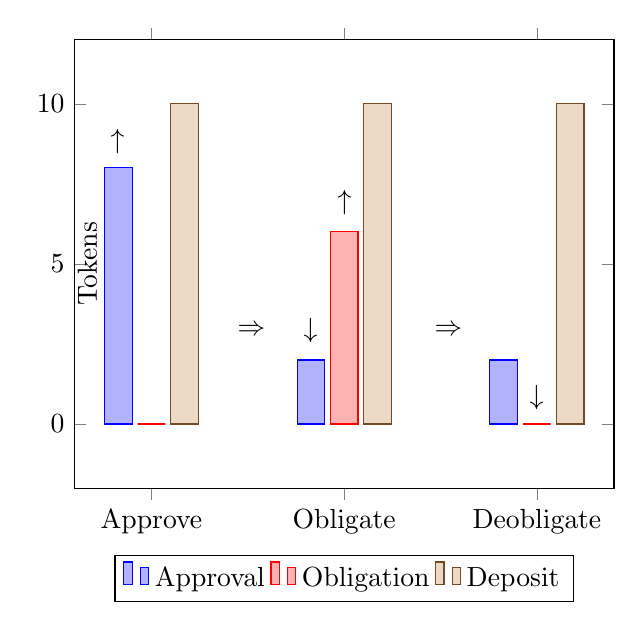
\begin{tikzpicture}
\begin{axis}[
    ybar,
    enlargelimits=0.2,
    legend style={at={(0.5,-0.15)},
      anchor=north,legend columns=-1},
    ylabel={Tokens},
    y label style={at={(axis description cs:.06,.5)}},
    symbolic x coords={Approve,Obligate,Deobligate},
    xtick=data,
    ]
\addplot coordinates {(Approve,8) (Obligate,2) (Deobligate,2)};
\addplot coordinates {(Approve,0) (Obligate,6) (Deobligate,0)};
\addplot coordinates {(Approve,10) (Obligate,10) (Deobligate,10)};
\legend{Approval,Obligation,Deposit}
\end{axis}
% Add the arrows
\node[] at (2.25,2) (x) {$\Rightarrow$};
\node[] at (4.75,2) (y) {$\Rightarrow$};
% Approve
\node[] at (.55,4.4) (x) {$\uparrow$};
% Obligate
\node[] at (3,2) (x) {$\downarrow$};
\node[] at (3.43,3.62) (x) {$\uparrow$};
% Deobligate
\node[] at (5.87,1.15) (x) {$\downarrow$};
\end{tikzpicture}
 \caption{Example stake lifecycle with deobligation}
 \label{fig:stake-deobligate}
\end{figure}

While an obligation is active, any \textbf{arbitration} permission holder can \textit{slash} the stake up to the amount of the obligation (see Figure \ref{fig:stake-slash}). We reiterate that this is a powerful ability and in most cases should be mediated by an appropriate extension (such as motions, described in Section \ref{sec:motions-and-disputes}).

\begin{figure}[h]
    \centering
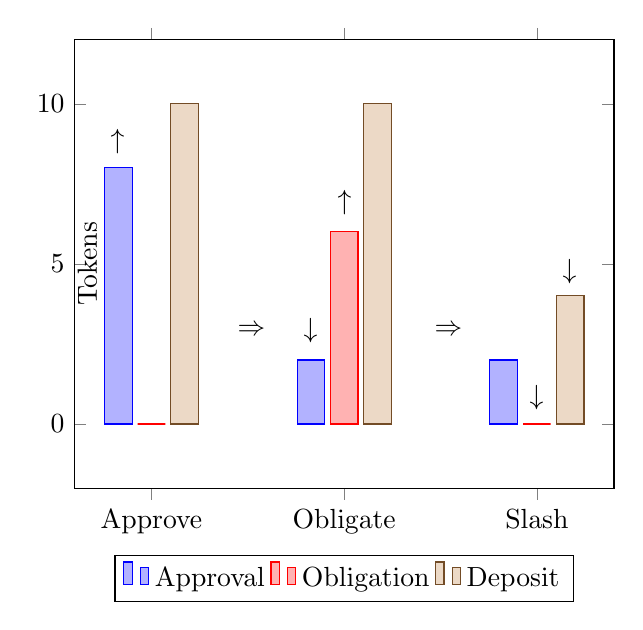
\begin{tikzpicture}
\begin{axis}[
    ybar,
    enlargelimits=0.2,
    legend style={at={(0.5,-0.15)},
      anchor=north,legend columns=-1},
    ylabel={Tokens},
    y label style={at={(axis description cs:.06,.5)}},
    symbolic x coords={Approve,Obligate,Slash},
    xtick=data,
    ]
\addplot coordinates {(Approve,8) (Obligate,2) (Slash,2)};
\addplot coordinates {(Approve,0) (Obligate,6) (Slash,0)};
\addplot coordinates {(Approve,10) (Obligate,10) (Slash,4)};
\legend{Approval,Obligation,Deposit}
\end{axis}
% Add the arrows
\node[] at (2.25,2) (x) {$\Rightarrow$};
\node[] at (4.75,2) (y) {$\Rightarrow$};
% Approve
\node[] at (.55,4.4) (x) {$\uparrow$};
% Obligate
\node[] at (3,2) (x) {$\downarrow$};
\node[] at (3.43,3.62) (x) {$\uparrow$};
% Slash
\node[] at (5.87,1.15) (x) {$\downarrow$};
\node[] at (6.29,2.75) (x) {$\downarrow$};
\end{tikzpicture}
 \caption{Example stake lifecycle with slashing}
 \label{fig:stake-slash}
\end{figure}

For reasons of security, approvals are keyed by \textit{domain}, as well as by address of approvee (i.e. \texttt{approve(approvee, domain, amount)}). Otherwise, a malicious actor could use \textit{any} arbitration permission holder in the colony to slash a stake, rather than arbitration permission holders in the intended domain inheritance path. However, because \texttt{TokenLocking} does not know about the domain structure of specific colonies, the obligations in \texttt{TokenLocking} are aggregates of all colony- and domain-specific obligations.

Overall, this design allows arbitration to be generalized and separated from the implementation of any particular extension: extensions obligate a stake (and define the period of obligation), while during that period separate arbitration processes can slash that stake.

\subsection{Upgradability and security}\label{subsec:upgradability}\label{sec:escape-hatches}

\subsubsection{Upgradability}

We foresee the Colony Network being continuously developed. Providing an upgrade path is important to allow people to use Colony without preventing themselves from using new features as they are added to the network.

We intend to allow colonies and tokens to be upgraded by using the pattern made available under the name EtherRouter \cite{EtherRouter}. This implementation uses two contracts in addition to the contract(s) providing the functionality implemented. The first additional contract is the \ascode{EtherRouter} contract, which passes on transactions --- via \ascode{delegatecall} --- to the contract that implements that function. The second additional contract is the \ascode{Resolver} contract, where the accounts of the contracts that implement the desired behaviour are defined. Whenever a transaction is received by the \ascode{EtherRouter} contract, it looks up the contract that implements that function (if any) in the \ascode{Resolver}, and then \ascode{delegatecall}s that contract.

In order to upgrade, new contracts are deployed with new functionality, and then contracts that the \ascode{Resolver} contract points to must be changed to point to these new contracts. In order to avoid a situation where the contract partially implements both old and new functionality,  a new instance of \ascode{Resolver} will be deployed for each upgrade, and then a single transaction can point \ascode{EtherRouter} at the new \ascode{Resolver}. From the perspective of the colony, an upgrade is then simply swapping out one address (the \ascode{Resolver}) for another.

The choice of upgrading the underlying Colony contract will always fall to the colony, and never the Colony Network. While the network is in control of what upgrades are available, they are not able to force any colony to upgrade the underlying contracts. The colony itself must decide that it wants to upgrade to a new version.

\subsubsection{Security}

While we aspire to bug-free contracts, bugs are inevitable, and so the adoption of a `defensive programming' mentality will limit the impact of any vulnerabilities that may be discovered in the deployed contracts.

The ultimate fallback is known as `recovery mode'. In this state, whitelisted accounts (those with the \textbf{recovery} permission) are able to access special functions that allow the state of the contract to be directly edited --- in practise, this will correspond to access to the functions to allow setting of variables, as well as being able to upgrade the contract. With the agreement of multiple whitelisted accounts, the contract will then be able to be taken out of recovery mode once the contract has been returned to a safe state. Removal from recovery mode requires the approval of multiple whitelisted accounts. This ensures that a single whitelisted account cannot, in a single transaction, enter recovery mode, make a malicious edit, and then exit recovery mode before the other parties on the whitelist have had a chance to react.

It is conceivable that colonies will be able to deactivate the recovery mode feature in the future, once the network and contracts have matured sufficiently. \\

In general, the contract may enter recovery mode due to:

\begin{itemize}
 \item A transaction from a whitelisted account signalling that the contract should enter recovery mode.
 \item Something that should always be true of the colony not being true --- for example, after an expenditure payout checking that the amount of funds promised to expenditures and not yet paid out is still less than the balance of the colony. If not, then abort the transaction and put the contract into recovery mode.
 \item A qualitative trigger suggesting something may be amiss --- perhaps too many tokens have been paid out in a short amount of time.
\end{itemize}

Any approvals from whitelisted accounts to leave recovery mode must be reset whenever a variable is edited. A whitelisted account agreeing to leave recovery mode records the timestamp at which the agreement occurred, and any change of variables also update a timestamp indicating the last edit. When attempting to leave recovery mode, only agreements made after the last edit are counted towards meeting the threshold.

The first \textbf{recovery} permission holder is set at colony creation and is the creator of the colony. Additional \textbf{recovery} permission holders can be added by the \textbf{root} permission.

\subsection{Arbitrary transactions}\label{sec:arbitrary-transaction}

Of course, it is possible that a colony will want to engage in some behaviour that we haven't foreseen, that could be implemented in a contract outside the control of the Colony Network (such as changing a parameter in a contract when the colony as a whole is responsible for governing that contract). To that end, we wish to have a mechanism by which a colony can create an arbitrary transaction on the blockchain to interact with contracts and tokens without requiring the network to explicitly support them. As they are powerful, such transactions should be rare occurrences requiring \textbf{root} authorization.
